\subsubsection{subfunction-oeDeleteHospital}

\label{RE-use-case-oeDeleteHospital}


goal is to delete an existing hospital in the system's post state and environment's post state.		  


\begin{usecase}
  \addheading{Use-Case Description}
  \addsingletwocolumnrow{Name}{oeDeleteHospital}
  \addsingletwocolumnrow{Scope}{system}
  \addsingletwocolumnrow{Level}{subfunction}
  
\addrowheading{Parameters}
\addnumberedsinglerow{AdtHospitalID: dtHospitalID}{}

\addrowheading{Primary actor(s)}
\addnumberedsinglerow{}{\msrcode{actAdministrator[active]}}



\addrowheading{Goal(s) description}
\addsinglerow{goal is to delete an existing hospital in the system's post state and environment's post state.}

\addrowheading{Protocol condition(s)}
\addnumberedsinglerow{}{
}

\addrowheading{Pre-condition(s)}
\addnumberedsinglerow{}{
}

\addrowheading{Main post-condition(s)}
\addnumberedsinglerow{}{
}

\addrowheading{Additional Information}
\addsinglerow{
none
}

\end{usecase} 

Figure \ref{fig:lu.uni.lassy.excalibur.examples.icrash-RE-UCD-uc-oeDeleteHospital}

\begin{figure}[htbp]
\begin{center}

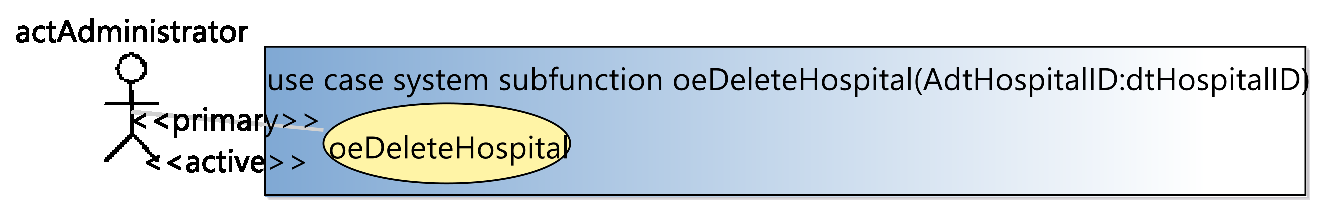
\includegraphics[
angle=0
]{./images-report-gen/usecase-model/subfunction/uc-oeDeleteHospital.eps}
\end{center}
\caption[lu.uni.lassy.excalibur.examples.icrash Use Case Diagram: uc-oeDeleteHospital]{}
\label{fig:lu.uni.lassy.excalibur.examples.icrash-RE-UCD-uc-oeDeleteHospital}
\end{figure}
\vspace{0.5cm}
